%-- Classical statistical model vs neural network-based --%
Time series analysis can be done in the frequency-domain or the time-domain. Classical time series analysis in the time-domain is based on Box-Jenkins work on regression modelling [cite Box and Jenkins]. In Box-Jenkins modelling an autoregressive integrated moving average-process (ARIMA-process) that models the temporal dependency is identified and fitted to data. This model can then be used for forecasting time series. However, ARIMA-processes are linear and can only handle data that can be made stationary. Autoregressive conditional heteroskedasticity (ARCH) models   

% Exponential smoothing/Holt-Winters
% Classification and regression trees
% STL decomposition
% Neural network
 

 black-box
 

\subsection{Recurrent Neural Networks}
Recurrent Neural Networks (RNNs) are a group of neural network that, in contrary to other neural networks, have loops in them. This gives them a memory which makes them good at handling sequential data. They are based on backpropagation ... \cite{Rumelhart1986}.

\begin{figure}[h]
    \centering
    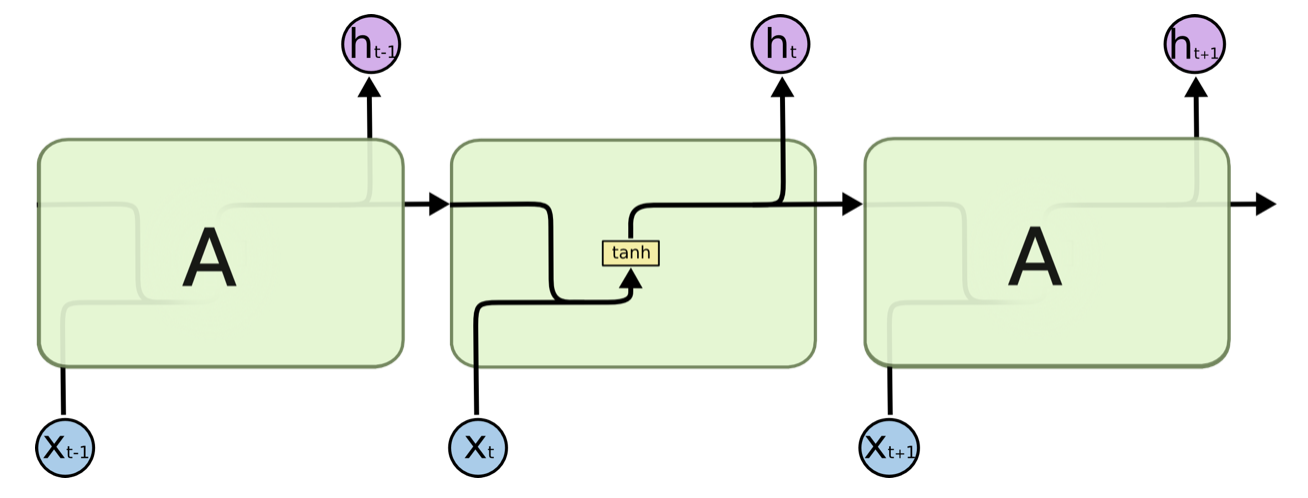
\includegraphics[width=0.5\textwidth]{Report/Chapters/Images/RNN.png}
    \caption{a nice plot}
    \label{fig:mesh1}
\end{figure}

% Vanishing gradient 
[cite Gradient Flow in Recurrent Nets: the Difficulty of Learning Long-Term Dependencies]



\subsubsection{Long Short-Term Memory}

\begin{figure}[h]
    \centering
    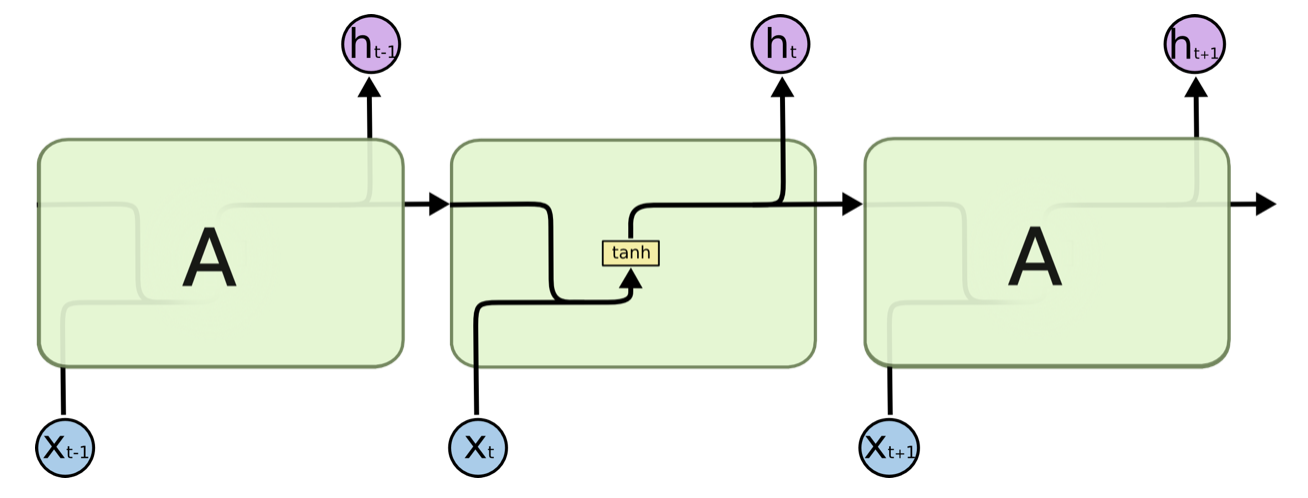
\includegraphics[width=0.5\textwidth]{Report/Chapters/Images/RNN.png}
    \caption{a nice plot}
    \label{fig:mesh1}
\end{figure}
